
\section{Kapitza-Dirac Prediction}

\noindent In 1933, Kapitza and Dirac proposed that the diffraction of an electron beam by a lattice formed of stationary electromagnetic waves could be observed. Because this relies on the process of stimulated emission, they predicted that the probability of such a process would be very low and would require a very intense light source to enhance the electron-photon interaction. Indeed, this technical feat had to wait 70 years for the advent of very powerful lasers. Figure~\ref{fig:Kapitza-Dirac} summarizes the principle of the experiment and its results.

\begin{figure}[H]
    \centering
    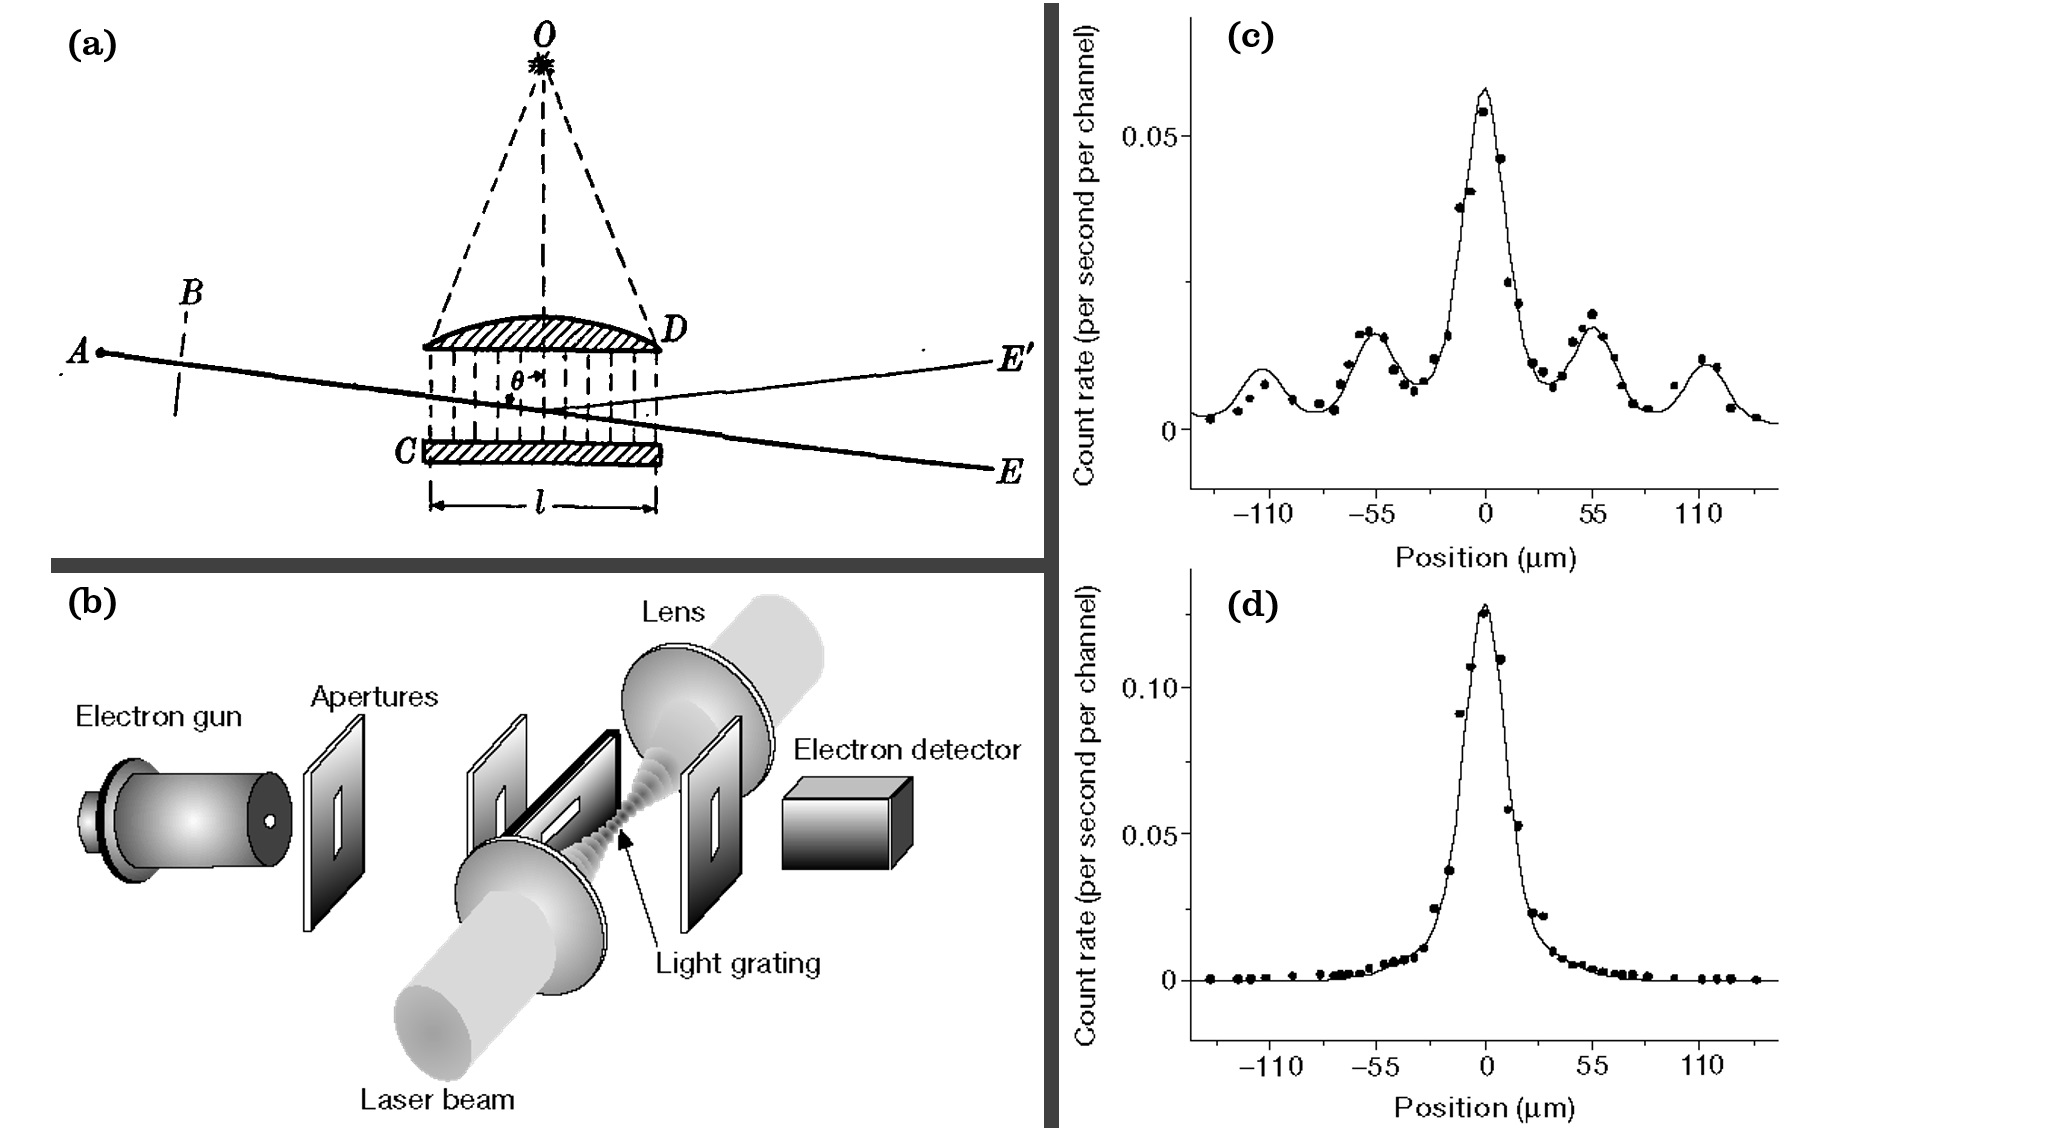
\includegraphics[width=\textwidth]{Kapitza-Dirac.jpg}
    \caption{Diffraction of massive particles by stationary electromagnetic waves. (a) Principle as described in Kapitza and Dirac's publication (1933). Electrons are emitted at $A$ and detected at $E^{\prime}$ when the lattice is created between lens $D$ and mirror $C$. When the light is off, the particles should be detected at $E$. (b) Experimental setup by Freimund and colleagues. (c) Interference fringes as seen by the detector at a distance of $24 \mathrm{~cm}$ from the lattice. The abscissa refers to the detector position. (d) Detected signal when the electromagnetic wave is turned off. Adapted from Nature, "Observation of the Kapitza-Dirac effect", Freimund, Kayvan, Aflatooni and Batelaan, \copyright \,2001.}
    \label{fig:Kapitza-Dirac}
\end{figure}

\noindent \textbf{1)} The electrons have an energy of about $380$ eV. What is the wavelength $\lambda_e$ of the incident electron beam?\\

\begin{breakbox}
    \noindent The wavelength is $\boxed{\lambda_e = \frac{2\pi}{k} = \frac{2\pi}{\sqrt{2m\epsilon_e}}\approx 0.6\ \text{Angstroms}.}$
\end{breakbox}

\medskip

\noindent \textbf{2)} The laser beam has a wavelength $\lambda_\nu=532$ nm. What is the energy of the photons? To achieve high power, the laser must operate with $10$ ns pulses, each carrying $0.2$ J. What is the photon flux (in $\mathrm{W/m^2 s}$) if the beam has a diameter of $125\ \mu \mathrm{m}$?\\

\begin{breakbox}
    \noindent Firstly, the energy of the photon is $\displaystyle \epsilon_{\nu} = \frac{2\pi\hbar c}{\lambda_{\nu}}\approx 3.7 \times 10^{-19}$ J $\approx 2.3$ eV. Secondly, the surface power density of the LASER is $\displaystyle d^{surf}_{P}=\frac{E_{pulse}}{\sigma \times \Delta t}$ with $\sigma$ the cross-section of the LASER beam, $\Delta t$ the time gap between each pulse, and $E_{pulse}$ the energy delivered by the LASER during a pulse. Thus, $\displaystyle d^{surf}_{P}=\frac{0.2}{10 \times 10^{-9}\times \pi \times (62.5 \times 10^{-6})^2} \approx 1.6 \times 10^{15} \: \mathrm{W/m^2}$. Finally, the photon flux is $\displaystyle \frac{d^{surf}_{P}}{\epsilon_{\nu}} = \frac{1.6 \times 10^{15}}{3.7 \times 10^{-19}} \approx 4.4 \times 10^{33} \: \mathrm{photons / (m^2 s)}$.
\end{breakbox}

\medskip

\noindent \textbf{3)} Justify the presence of a first-order diffraction peak at $55 \mu \mathrm{m}$ using the diffraction law $d \sin \theta=n \lambda$, where $d$ is the lattice period, $\lambda$ is the wavelength of the incident radiation, and $\theta$ is the diffraction angle.\\

\begin{breakbox}
    \noindent The light gridding (i.e., two-dimensional lattice) is created by the intensity of the diffracted radiation. Thus, the period is half a wavelength $\displaystyle d = \frac{\lambda_{\nu}}{2} = 532/2$ nm. Using the diffraction law for the first order ($n = 1$), we find that the angle corresponding to the first diffraction peak is $\displaystyle \theta_1 = \frac{2 \times 0.6 \times 10^{-10}}{532 \times 10^{-9}} \approx 0.226 \times 10^{-3}$ rad, and the detector for this first maximum is placed at $x_1 = 0.226 \times 10^{-3} \times 0.24 \approx 54 \mathrm{\mu m}$.
\end{breakbox}

